\section{Program synthesis}

Program synthesis is a process of automatic program generation, in accordance with some specific goals.

% subsections:
\subsection{Synthesis of simple program using Z3 SMT-solver}
\label{synth_mult}

\renewcommand{\CURPATH}{synth/pgm/load}

Sometimes, multiplication operation can be replaced with a several operations of shifting/addition/subtraction.
Compilers do so, because pack of instructions can be executed faster.

For example, multiplication by 19 is replaced by GCC 5.4 with pair of instructions: \TT{lea edx, [eax+eax*8]} and\\
\TT{lea eax, [eax+edx*2]}.
This is sometimes also called ``superoptimization''.

Let's see if we can find a shortest possible instructions pack for some specified multiplier.

As I've already wrote once, SMT-solver can be seen as a solver of huge systems of equations.
The task is to construct such system of equations, which, when solved, could produce a short program.
I will use electronics analogy here, it can make things a little simpler.

First of all, what our program will be consting of? There will be 3 operations allowed: ADD/SUB/SHL.
Only registers allowed as operands, except for the second operand of SHL (which could be in 1..31 range).
Each register will be assigned only once (as in \ac{SSA}).

And there will be some ``magic block'', which takes all previous register states, it also takes operation type,
operands and produces a value of next register's state.

\begin{lstlisting}
	        op ------------+
	        op1_reg -----+ |
	        op2_reg ---+ | |
	                   | | |
	                   v v v
	             +---------------+
	             |               |
	registers -> |               | -> new register's state
	             |               |
	             +---------------+
\end{lstlisting}

Now let's take a look on our schematics on top level:

\begin{lstlisting}
	0 -> blk -> blk -> blk .. -> blk -> 0

	1 -> blk -> blk -> blk .. -> blk -> multiplier
\end{lstlisting}

Each block takes previous state of registers and produces new states.
There are two chains.
First chain takes 0 as state of R0 at the very beginning, and the chain is supposed to produce 0 at the end
(since zero multiplied by any value is still zero).
The second chain takes 1 and must produce multiplier as the state of very last register
(since 1 multiplied by multiplier must equal to multiplier).

Each block is ``controlled'' by operation type, operands, etc.
For each column, there is each own set.

Now you can view these two chains as two equations.
The ultimate goal is to find such state of all operation types and operands, so the first chain will equal to 0,
and the second to multiplier.

Let's also take a look into ``magic block'' inside:

\begin{lstlisting}
	                op1_reg         op
	                   |            v
	                   v         +-----+
	registers ---> selector1 --> | ADD |
	           +                 | SUB | ---> result
	           |                 | SHL |
	           +-> selector2 --> +-----+
	                  ^             ^
	                  |             |
	               op2_reg       op2_imm
\end{lstlisting}

Each selector can be viewed as a simple multipositional switch.
If operation is SHL, a value in range of 1..31 is used as second operand.

So you can imagine this electric circuit and your goal is to turn all switches in such a state, so two chains
will have 0 and multiplier on output.
This sounds like logic puzzle in some way.
Now we will try to use Z3 to solve this puzzle.

First, we define all varibles:

\begin{lstlisting}
R=[[BitVec('S_s%d_c%d' % (s, c), 32) for s in range(MAX_STEPS)] for c in range (CHAINS)]
op=[Int('op_s%d' % s) for s in range(MAX_STEPS)]
op1_reg=[Int('op1_reg_s%d' % s) for s in range(MAX_STEPS)]
op2_reg=[Int('op2_reg_s%d' % s) for s in range(MAX_STEPS)]
op2_imm=[BitVec('op2_imm_s%d' % s, 32) for s in range(MAX_STEPS)]
\end{lstlisting}

R[][] is registers state for each chain and each step.\\
On contrary, \TT{op}/\TT{op1\_reg}/\TT{op2\_reg}/\TT{op2\_imm} variables are defined for each step, but for both chains,
since both chains at each column has the same operation/operands.

Now we must limit count of operations, and also, register's number for each step must not be bigger than step number,
in other words, instruction at each step is allowed to access only registers which were already set before:

\begin{lstlisting}
for s in range(1, STEPS):
    # for each step
    sl.add(And(op[s]>=0, op[s]<=2))
    sl.add(And(op1_reg[s]>=0, op1_reg[s]<s))
    sl.add(And(op2_reg[s]>=0, op2_reg[s]<s))
    sl.add(And(op2_imm[s]>=1, op2_imm[s]<=31))
\end{lstlisting}

Fix register of first step for both chains:

\begin{lstlisting}
for c in range(CHAINS):
    # for each chain:
    sl.add(R[c][0]==chain_inputs[c])
    sl.add(R[c][STEPS-1]==chain_inputs[c]*multiplier)
\end{lstlisting}

Now let's add ``magic blocks'':

\begin{lstlisting}
for s in range(1, STEPS):
    sl.add(R[c][s]==simulate_op(R,c, op[s], op1_reg[s], op2_reg[s], op2_imm[s]))
\end{lstlisting}

Now how ``magic block'' is defined?

\begin{lstlisting}
def selector(R, c, s):
    # for all MAX_STEPS:
    return If(s==0, R[c][0],
	    If(s==1, R[c][1],
            If(s==2, R[c][2],
	    If(s==3, R[c][3],
            If(s==4, R[c][4],
            If(s==5, R[c][5],
	    If(s==6, R[c][6],
            If(s==7, R[c][7],
	    If(s==8, R[c][8],
            If(s==9, R[c][9],
	        0)))))))))) # default

def simulate_op(R, c, op, op1_reg, op2_reg, op2_imm):
    op1_val=selector(R,c,op1_reg)
    return If(op==0, op1_val + selector(R, c, op2_reg),
	   If(op==1, op1_val - selector(R, c, op2_reg),
           If(op==2, op1_val << op2_imm,
	       0))) # default
\end{lstlisting}

This is very important to understand: if the operation is ADD/SUB, \TT{op2\_imm}'s value is just ignored.
Otherwise, if operation is SHL, value of \TT{op2\_reg} is ignored.
Just like in case of digital circuit.

The code: \url{\GitHubBlobMasterURL/\CURPATH/mult.py}

Now let's see how it works:

\begin{lstlisting}
% ./mult.py 12
multiplier= 12
attempt, STEPS= 2
unsat
attempt, STEPS= 3
unsat
attempt, STEPS= 4
sat!
r1=SHL r0, 2
r2=SHL r1, 1
r3=ADD r1, r2
tests are OK
\end{lstlisting}

The first step is always a step containing 0/1, or, r0.
So when our solver reporting about 4 steps, this means 3 instructions.

Something harder:

\begin{lstlisting}
% ./mult.py 123
multiplier= 123
attempt, STEPS= 2
unsat
attempt, STEPS= 3
unsat
attempt, STEPS= 4
unsat
attempt, STEPS= 5
sat!
r1=SHL r0, 2
r2=SHL r1, 5
r3=SUB r2, r1
r4=SUB r3, r0
tests are OK
\end{lstlisting}

Now the code multiplying by 1234:

\begin{lstlisting}
r1=SHL r0, 6
r2=ADD r0, r1
r3=ADD r2, r1
r4=SHL r2, 4
r5=ADD r2, r3
r6=ADD r5, r4
\end{lstlisting}

Looks great, but it took $\approx 23$ seconds to find it on my Intel Xeon CPU E31220 @ 3.10GHz.
I agree, this is far from practical usage.
Also, I'm not quite sure that this piece of code will work faster than a single multiplication instruction.
But anyway, it's a good demonstration of SMT solvers capabilities.

The code multiplying by 12345 ($\approx 150$ seconds):

\begin{lstlisting}
r1=SHL r0, 5
r2=SHL r0, 3
r3=SUB r2, r1
r4=SUB r1, r3
r5=SHL r3, 9
r6=SUB r4, r5
r7=ADD r0, r6
\end{lstlisting}

Multiplication by 123456 ($\approx 8$ minutes!):

\begin{lstlisting}
r1=SHL r0, 9
r2=SHL r0, 13
r3=SHL r0, 2
r4=SUB r1, r2
r5=SUB r3, r4
r6=SHL r5, 4
r7=ADD r1, r6
\end{lstlisting}

\subsubsection{Few notes}

I've removed SHR instruction support, simply because the code multiplying by a constant makes no use of it.
Even more: it's not a problem to add support of constants as second operand for all instructions,
but again, you wouldn't find a piece of code which does this job and uses some additional constants.
Or maybe I wrong?

Of course, for another job you'll need to add support of constants and other operations.
But at the same time, it will work slower and slower.
So I had to keep \ac{ISA} of this toy \ac{CPU} as compact as possible.

\subsubsection{The code}

\url{\GitHubTreeMasterURL/\CURPATH}


\subsection{Rockey dongle: finding unknown algorithm using only input/output pairs}

\renewcommand{\CURPATH}{synth/pgm/rockey}

(This text was first published in August 2012 in my blog: \url{http://blog.yurichev.com/node/71}.)

Some smartcards can execute Java or .NET code - that's the way to hide your sensitive algorithm
into chip that is very hard to break (decapsulate).
For example, one may encrypt/decrypt data files by hidden crypto algorithm rendering software
piracy of such software close to impossible---an encrypted date file created on software with connected smartcard
would be impossible to decrypt on cracked version of the same software.
(This leads to many nuisances, though.)

That's what is called \emph{black box}.

Some software protection dongles offers this functionality too.
One example is Rockey 4\footnote{\url{http://www.rockey.nl/en/rockey.html}}.

\begin{figure}[H]
\centering
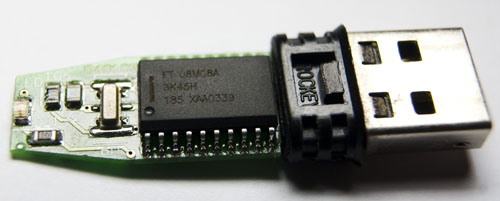
\includegraphics[scale=2]{\CURPATH/rockey_4.jpg}
\caption{Rockey 4 dongle}
\end{figure}

This is a small dongle connected via USB. Is contain some user-defined memory but also memory for user algorithms.

The virtual (toy) CPU for these algorithms is very simple: it offer only 8 16-bit registers
(however, only 4 can be set and read) and 8 operations
(addition, subtractation, cyclic left shifting, multiplication, OR, XOR, AND, negation).

Second instruction argument can be a constant (from 0 to 63) instead of register.

Each algorithm is described by string like \\
\TT{A=A+B, B=C*13, D=D\^{}A, C=B*55, C=C\&A, D=D|A, A=A*9, A=A\&B}.

There are no memory, stack, conditional/unconditional jumps, etc.

Each algorithm, obviously, can't have side effects, so they are actually \emph{pure functions}
and their results can be \emph{memoized}.

By the way, as it has been mentioned in Rockey 4 manual, first and last instruction cannot have constants.
Maybe that's because these fields used for some internal data:
each algorithm start and end should be marked somehow internally anyway.

Would it be possible to reveal hidden impossible-to-read algorithm only by recording input/output dongle traffic?
Common sense tell us ``no''. But we can try anyway.

Since, my goal wasn't to break into some Rockey-protected software,
I was interesting only in limits (which algorithms could we find),
so I make some things simpler: we will work with only 4 16-bit registers,
and there will be only 6 operations (add, subtract, multiply, OR, XOR, AND).

Let's first calculate, how much information will be used in brute-force case.

There are 384 of all possible instructions in \TT{reg=reg,op,reg} format for 4 registers and 6 operations,
and also 6144 instructions in \TT{reg=reg,op,constant} format.
Remember that constant limited to 63 as maximal value? That help us for a little.

So, there are 6528 of all possible instructions.
This mean, there are $\approx 1.1 \cdot 10^{19}$ 5-instruction algorithms.
That's too much.

How can we express each instruction as system of equations?
While remembering some school mathematics, I wrote this:

\begin{lstlisting}
Function one\_step()=

# Each Bx is integer, but may be only 0 or 1.

# only one of B1..B4 and B5..B9 can be set
reg1=B1*A + B2*B + B3*C + B4*D
reg_or_constant2=B5*A + B6*B + B7*C + B8*D + B9*constant
reg1 should not be equal to reg_or_constant2

# Only one of B10..B15 can be set
result=result+B10*(reg1*reg2)
result=result+B11*(reg1^reg2)
result=result+B12*(reg1+reg2)
result=result+B13*(reg1-reg2)
result=result+B14*(reg1|reg2)
result=result+B15*(reg1&reg2)

B16 - true if register isn't updated in this part
B17 - true if register is updated in this part
(B16 cannot be equal to B17)
A=B16*A + B17*result
B=B18*A + B19*result
C=B20*A + B21*result
D=B22*A + B23*result
\end{lstlisting}

That's how we can express each instruction in algorithm.

5-instructions algorithm can be expressed like this:\\
\TT{one\_step (one\_step (one\_step (one\_step (one\_step (input\_registers)))))}.

Let's also add five known input/output pairs and we'll get system of equations like this:

\begin{lstlisting}
one_step (one_step (one_step (one_step (one_step (input_1)))))==output_1
one_step (one_step (one_step (one_step (one_step (input_2)))))==output_2
one_step (one_step (one_step (one_step (one_step (input_3)))))==output_3
one_step (one_step (one_step (one_step (one_step (input_4)))))==output_4
.. etc
\end{lstlisting}

So the question now is to find $5 \cdot 23$ boolean values satisfying known input/output pairs.

I wrote small utility to probe Rockey 4 algorithm with random numbers, it produce results in form:

\begin{lstlisting}
RY_CALCULATE1: (input) p1=30760 p2=18484 p3=41200 p4=61741 (output) p1=49244 p2=11312 p3=27587 p4=12657
RY_CALCULATE1: (input) p1=51139 p2=7852 p3=53038 p4=49378 (output) p1=58991 p2=34134 p3=40662 p4=9869
RY_CALCULATE1: (input) p1=60086 p2=52001 p3=13352 p4=45313 (output) p1=46551 p2=42504 p3=61472 p4=1238
RY_CALCULATE1: (input) p1=48318 p2=6531 p3=51997 p4=30907 (output) p1=54849 p2=20601 p3=31271 p4=44794
\end{lstlisting}

p1/p2/p3/p4 are just another names for A/B/C/D registers.

Now let's start with Z3. We will need to express Rockey 4 toy CPU in Z3Py (Z3 Python \ac{API}) terms.

It can be said, my Python script is divided into two parts: 

\begin{itemize}
\item constraint definitions (like, \emph{output\_1 should be $n$ for input\_1=m},
\emph{constant cannot be greater than 63}, etc); 

\item functions constructing system of equations.
\end{itemize}

This piece of code define some kind of \emph{structure} consisting of 4 named 16-bit variables,
each represent register in our toy CPU.

\begin{lstlisting}
Registers_State=Datatype ('Registers_State')
Registers_State.declare('cons', ('A', BitVecSort(16)), ('B', BitVecSort(16)), ('C', BitVecSort(16)), ('D', BitVecSort(16)))
Registers_State=Registers_State.create()
\end{lstlisting}

These enumerations define two new types (or \emph{sorts} in Z3's terminology):

\begin{lstlisting}
Operation, (OP_MULT, OP_MINUS, OP_PLUS, OP_XOR, OP_OR, OP_AND) = EnumSort('Operation', ('OP_MULT', 'OP_MINUS', 'OP_PLUS', 'OP_XOR', 'OP_OR', 'OP_AND'))

Register, (A, B, C, D) = EnumSort('Register', ('A', 'B', 'C', 'D'))
\end{lstlisting}

This part is very important, it defines all variables in our system of equations. 
\TT{op\_step} is type of operation in instruction.
\TT{reg\_or\_constant} is selector between register and constant in second argument ---
\emph{False} if it's a register and \emph{True} if it's a constant. 
\TT{reg\_step} is a destination register of this instruction. 
\TT{reg1\_step} and \TT{reg2\_step} are just registers at arg1 and arg2. 
\TT{constant\_step} is constant (in case it's used in instruction instead of arg2).

\begin{lstlisting}
op_step=[Const('op_step%s' % i, Operation) for i in range(STEPS)]
reg_or_constant_step=[Bool('reg_or_constant_step%s' % i) for i in range(STEPS)]
reg_step=[Const('reg_step%s' % i, Register) for i in range(STEPS)]
reg1_step=[Const('reg1_step%s' % i, Register) for i in range(STEPS)]
reg2_step=[Const('reg2_step%s' % i, Register) for i in range(STEPS)]
constant_step = [BitVec('constant_step%s' % i, 16) for i in range(STEPS)]
\end{lstlisting}

Adding constraints is very simple. Remember, I wrote that each constant cannot be larger than 63?

\begin{lstlisting}
# according to Rockey 4 dongle manual, arg2 in first and last instructions cannot be a constant
s.add (reg_or_constant_step[0]==False)
s.add (reg_or_constant_step[STEPS-1]==False)

...

for x in range(STEPS):
   s.add (constant_step[x]>=0, constant_step[x]<=63)
\end{lstlisting}

Known input/output values are added as constraints too.

Now let's see how to construct our system of equations:

\begin{lstlisting}
# Register, Registers_State -> int
def register_selector (register, input_registers):
    return If(register==A, Registers_State.A(input_registers),
           If(register==B, Registers_State.B(input_registers), 
           If(register==C, Registers_State.C(input_registers), 
           If(register==D, Registers_State.D(input_registers), 
                           0)))) # default
\end{lstlisting}

This function returning corresponding register value from \emph{structure}.
Needless to say, the code above is not executed. 
\TT{If()} is Z3Py function. 
The code only declares the function, which will be used in another. 
Expression declaration resembling LISP \ac{PL} in some way.

Here is another function where \TT{register\_selector()} is used:

\begin{lstlisting}
# Bool, Register, Registers_State, int -> int
def register_or_constant_selector (register_or_constant, register, input_registers, constant): 
    return If(register_or_constant==False, register_selector(register, input_registers), constant)
\end{lstlisting}

The code here is never executed too. 
It only constructs one small piece of very big expression. 
But for the sake of simplicity, one can think all these functions will be called during bruteforce search, many times,
at fastest possible speed.

\begin{lstlisting}
# Operation, Bool, Register, Register, Int, Registers_State -> int
def one_op (op, register_or_constant, reg1, reg2, constant, input_registers):
    arg1=register_selector(reg1, input_registers)
    arg2=register_or_constant_selector (register_or_constant, reg2, input_registers, constant)
    return If(op==OP_MULT,   arg1*arg2,
           If(op==OP_MINUS,  arg1-arg2,
           If(op==OP_PLUS,   arg1+arg2, 
           If(op==OP_XOR,    arg1^arg2, 
           If(op==OP_OR,     arg1|arg2, 
           If(op==OP_AND,    arg1&arg2, 
                          0)))))) # default
\end{lstlisting}

Here is the expression describing each instruction. 
\TT{new\_val} will be assigned to destination register,
while all other registers' values are copied from input registers' state:

\begin{lstlisting}
# Bool, Register, Operation, Register, Register, Int, Registers_State -> Registers_State
def one_step (register_or_constant, register_assigned_in_this_step, op, reg1, reg2, constant, input_registers):
    new_val=one_op(op, register_or_constant, reg1, reg2, constant, input_registers)
    return If (register_assigned_in_this_step==A, Registers_State.cons (new_val,
                                   Registers_State.B(input_registers), 
                                   Registers_State.C(input_registers), 
                                   Registers_State.D(input_registers)),
           If (register_assigned_in_this_step==B, Registers_State.cons (Registers_State.A(input_registers), 
                                   new_val,
                                   Registers_State.C(input_registers),
                                   Registers_State.D(input_registers)), 
           If (register_assigned_in_this_step==C, Registers_State.cons (Registers_State.A(input_registers), 
                                   Registers_State.B(input_registers), 
                                   new_val,
                                   Registers_State.D(input_registers)), 
           If (register_assigned_in_this_step==D, Registers_State.cons (Registers_State.A(input_registers), 
                                   Registers_State.B(input_registers), 
                                   Registers_State.C(input_registers), 
                                   new_val),
                                                  Registers_State.cons(0,0,0,0))))) # default
\end{lstlisting}

This is the last function describing a whole $n$-step program:

\begin{lstlisting}
def program(input_registers, STEPS):
    cur_input=input_registers
    for x in range(STEPS):
        cur_input=one_step (reg_or_constant_step[x], reg_step[x], op_step[x], reg1_step[x], reg2_step[x], constant_step[x], cur_input)
    return cur_input
\end{lstlisting}

Again, for the sake of simplicity, it can be said, now Z3 will try each possible
registers/operations/constants against this expression to find such combination which satisfy all input/output pairs. 
Sounds absurdic, but this is close to reality.
SAT/SMT-solvers indeed tries them all.
But the trick is to prune search tree as early as possible, so it will work for some reasonable time.
And this is hardest problem for solvers.

Now let's start with very simple 3-step algorithm: \TT{B=A\^{}D, C=D*D, D=A*C}.
Please note: register \TT{A} left unchanged.
I programmed Rockey 4 dongle with the algorithm, and recorded algorithm outputs are:

\begin{lstlisting}
RY_CALCULATE1: (input) p1=8803 p2=59946 p3=36002 p4=44743 (output) p1=8803 p2=36004 p3=7857 p4=24691
RY_CALCULATE1: (input) p1=5814 p2=55512 p3=52155 p4=55813 (output) p1=5814 p2=52403 p3=33817 p4=4038
RY_CALCULATE1: (input) p1=25206 p2=2097 p3=55906 p4=22705 (output) p1=25206 p2=15047 p3=10849 p4=43702
RY_CALCULATE1: (input) p1=10044 p2=14647 p3=27923 p4=7325 (output) p1=10044 p2=15265 p3=47177 p4=20508
RY_CALCULATE1: (input) p1=15267 p2=2690 p3=47355 p4=56073 (output) p1=15267 p2=57514 p3=26193 p4=53395
\end{lstlisting}

It took about one second and only 5 pairs above to find algorithm
(on my quad-core Xeon E3-1220 3.1GHz, however, Z3 solver working in single-thread mode):

\begin{lstlisting}
B = A ^ D
C = D * D
D = C * A
\end{lstlisting}

Note the last instruction: \TT{C} and \TT{A} registers are swapped comparing to version I wrote by hand. 
But of course, this instruction is working in the same way, because multiplication is commutative operation.

Now if I try to find 4-step program satisfying to these values, my script will offer this:

\begin{lstlisting}
B = A ^ D
C = D * D
D = A * C
A = A | A
\end{lstlisting}

\dots and that's really fun, because the last instruction do nothing with value in register \TT{A},
it's like \ac{NOP}---but still, algorithm is correct for all values given.

Here is another 5-step algorithm: \TT{B=B\^{}D, C=A*22, A=B*19, A=A\&42, D=B\&C} and values:

\begin{lstlisting}
RY_CALCULATE1: (input) p1=61876 p2=28737 p3=28636 p4=50362 (output) p1=32 p2=46331 p3=50552 p4=33912
RY_CALCULATE1: (input) p1=46843 p2=43355 p3=39078 p4=24552 (output) p1=8 p2=63155 p3=47506 p4=45202
RY_CALCULATE1: (input) p1=22425 p2=51432 p3=40836 p4=14260 (output) p1=0 p2=65372 p3=34598 p4=34564
RY_CALCULATE1: (input) p1=44214 p2=45766 p3=19778 p4=59924 (output) p1=2 p2=22738 p3=55204 p4=20608
RY_CALCULATE1: (input) p1=27348 p2=49060 p3=31736 p4=59576 (output) p1=0 p2=22300 p3=11832 p4=1560
\end{lstlisting}

It took 37 seconds and we've got:

\begin{lstlisting}
B = D ^ B
C = A * 22
A = B * 19
A = A & 42
D = C & B
\end{lstlisting}

\TT{A=A\&42} was correctly deduced (look at these five p1's at output (assigned to output \TT{A} register): 32,8,0,2,0)

6-step algorithm \TT{A=A+B, B=C*13, D=D\^{}A, C=C\&A, D=D|B, A=A\&B} and values:

\begin{lstlisting}
RY_CALCULATE1: (input) p1=4110 p2=35411 p3=54308 p4=47077 (output) p1=32832 p2=50644 p3=36896 p4=60884
RY_CALCULATE1: (input) p1=12038 p2=7312 p3=39626 p4=47017 (output) p1=18434 p2=56386 p3=2690 p4=64639
RY_CALCULATE1: (input) p1=48763 p2=27663 p3=12485 p4=20563 (output) p1=10752 p2=31233 p3=8320 p4=31449
RY_CALCULATE1: (input) p1=33174 p2=38937 p3=54005 p4=38871 (output) p1=4129 p2=46705 p3=4261 p4=48761
RY_CALCULATE1: (input) p1=46587 p2=36275 p3=6090 p4=63976 (output) p1=258 p2=13634 p3=906 p4=48966
\end{lstlisting}

90 seconds and we've got:

\begin{lstlisting}
A = A + B
B = C * 13
D = D ^ A
D = B | D
C = C & A
A = B & A
\end{lstlisting}

But that was simple, however. 
Some 6-step algorithms are not possible to find, for example: \\
\TT{A=A\^{}B, A=A*9, A=A\^{}C, A=A*19, A=A\^{}D, A=A\&B}.
Solver was working too long (up to several hours), so I didn't even know is it possible to find it anyway.

\subsubsection{Conclusion}

This is in fact an exercise in program synthesis.

Some short algorithms for tiny \ac{CPU}s are really possible to find using so small set set of data.
Of course it's still not possible to reveal some complex algorithm,
but this method definitely should not be ignored.

\subsection{The files}

Rockey 4 dongle programmer and reader, Rockey 4 manual, Z3Py script for finding algorithms, input/output pairs:
\url{\GitHubTreeMasterURL/\CURPATH}

\subsubsection{Further work}

Perhaps, constructing LISP-like S-expression can be better than a program for toy-level CPU.

It's also possible to start with smaller constants and then proceed to bigger.
This is somewhat similar to increasing password length in password brute-force cracking.

\subsubsection{Exercise}

\url{https://challenges.re/25/}.


\subsection{TAOCP 7.1.3 Exercise 198, UTF-8 encoding and program synthesis by sketching}

\renewcommand{\CURPATH}{synth/pgm/TAOCP_713_198}

Found this exercise in TAOCP 7.1.3 (Bitwise Tricks and Techniques):

% TODO: border
\begin{figure}[H]
\centering
\frame{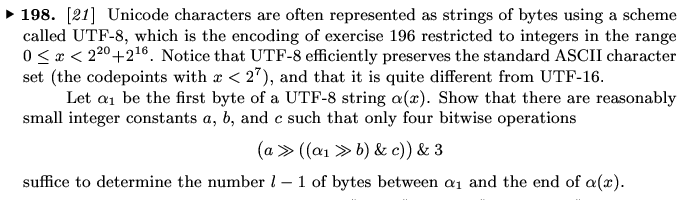
\includegraphics[scale=0.75]{\CURPATH/TAOCP_713_198.png}}
\caption{Exercise from TAOCP book}
\end{figure}

This is like program synthesis by sketching: you give a sketch with several ``holes'' missing and ask some
automated software to fill the ``holes''.
In our case, $a$, $b$ and $c$ are ``holes''.

Let's find them using Z3:

\lstinputlisting[style=custompy]{\CURPATH/198.py}

I tried various bit widths for a, b and c and found that 22 bits are enough.
I've lots of results like:

\begin{lstlisting}
...

a,b,c = 0x250100 0x3 0x381416
a,b,c = 0x258100 0x3 0x381416
a,b,c = 0x258900 0x3 0x381416
a,b,c = 0x250900 0x3 0x381416
a,b,c = 0x251100 0x3 0x381416
a,b,c = 0x259100 0x3 0x381416
a,b,c = 0x259100 0x3 0x389416
a,b,c = 0x251100 0x3 0x389416
a,b,c = 0x251100 0x3 0x189416
a,b,c = 0x259100 0x3 0x189416
a,b,c = 0x259100 0x3 0x189016

...
\end{lstlisting}

It seems that several least significant bits of a and c are not used.
After little experimentation, I've come to this:

\begin{lstlisting}
...

# make a,c more aesthetically appealing:
s.add((a&0xffff)==0)
s.add((c&0xffff00)==0)

...
\end{lstlisting}

And the results:

\begin{lstlisting}
a,b,c = 0x250000 0x3 0x36
a,b,c = 0x250000 0x3 0x16
a,b,c = 0x250000 0x3 0x96
a,b,c = 0x250000 0x3 0xd6
a,b,c = 0x250000 0x3 0xf6
a,b,c = 0x250000 0x3 0x76
a,b,c = 0x250000 0x3 0xb6
a,b,c = 0x250000 0x3 0x56
results total= 8
\end{lstlisting}

Pick any.

But how it works?
Its operation is very similar to the bitwise trick related to leading/trailing zero bits counting based on De Bruijn sequences.
Read more about it in \MathForProg.


\subsection{TAOCP 7.1.3 Exercise 203, MMIX MOR instruction and program synthesis by sketching}

\renewcommand{\CURPATH}{synth/pgm/TAOCP_713_203}

Found this exercise in TAOCP 7.1.3 (Bitwise Tricks and Techniques):

% TODO: border
\begin{figure}[H]
\centering
\frame{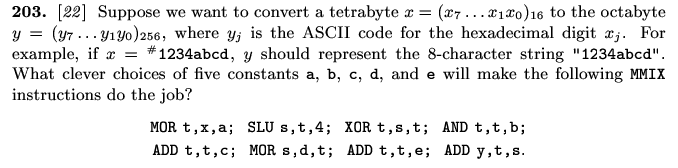
\includegraphics[scale=0.7]{\CURPATH/203q.png}}
\caption{Screenshot from TAOCP book}
\end{figure}

What is MOR instruction in MMIX?

\begin{figure}[H]
\centering
\frame{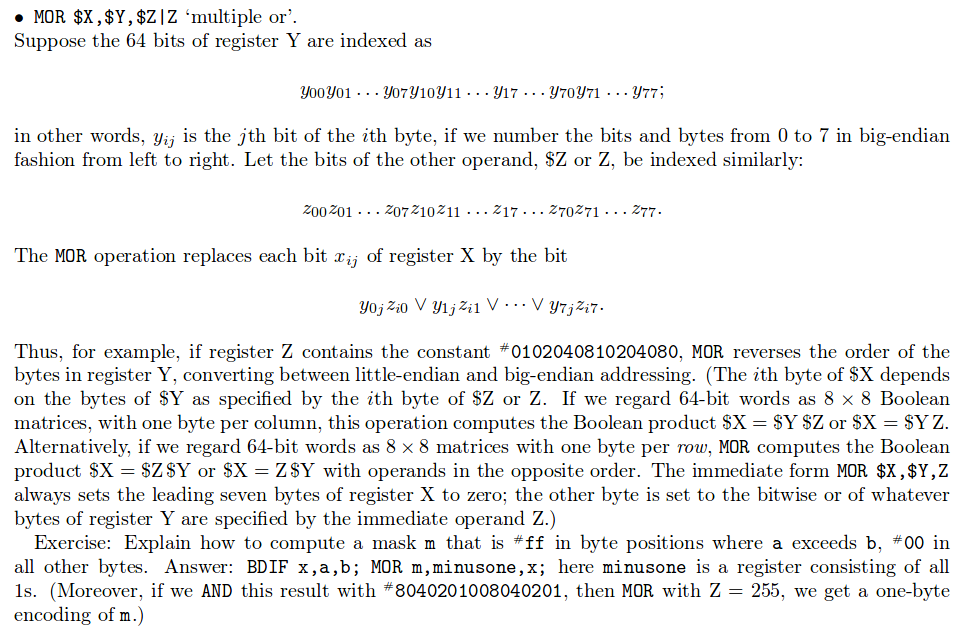
\includegraphics[scale=0.55]{\CURPATH/MOR.png}}
\caption{Screenshot from the MMIX book}
\end{figure}

( \url{http://mmix.cs.hm.edu/doc/mmix-doc.pdf} )

Let's try to solve. We create two functions. First has MOR instructions simulation + the program from TAOCP.
The second is a naive implementation.
Then we add ``forall'' quantifier: for all inputs, both functions must produce the same result.
\textbf{But}, we don't know a/b/c/d/e/f and ask Z3 SMT-solver to

\lstinputlisting[style=custompy]{\CURPATH/v1.py}

Very slow, it takes several hours on my venerable Intel Quad-Core Xeon E3-1220 3.10GHz but found at least one solution:

\begin{lstlisting}
a,b,c,d,e = 8000400020001 f0f0f0f0f0f0f0f 56d656d616969616 411a00000000 bf3fbf3fff7f8000
\end{lstlisting}

\dots which is correct (I've wrote bruteforce checker, here: \url{\GitHubBlobMasterURL/\CURPATH/check.c}.

D.Knuth's TAOCP also has answers:

\begin{figure}[H]
\centering
\frame{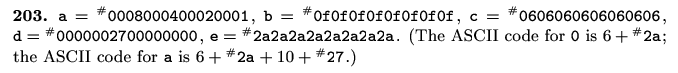
\includegraphics[scale=0.6]{\CURPATH/203a.png}}
\caption{Screenshot from TAOCP book}
\end{figure}

\dots which are different, but also correct.

What if a==0x0008000400020001 always?
I'm adding a new constraint:

\begin{lstlisting}
s.add(a==0x0008000400020001)
\end{lstlisting}

We've getting many results (much faster, and also correct):

\begin{lstlisting}
...

a,b,c,d,e = 8000400020001 7f0fcf0fcf0f7f0f 1616d6d656561656 8680522903020000 eeeda9aa2e2eee2f
a,b,c,d,e = 8000400020001 7f0fcf0fcf0f6f0f 1616d6d656561656 8680522903020000 eeeda9aa2e2eee2f
a,b,c,d,e = 8000400020001 7f0fcf0fdf0f6f0f 1616d6d656561656 8680522903020000 eeeda9aa2e2eee2f
a,b,c,d,e = 8000400020001 5f0fcf0fdf0f6f0f 1616d6d656561656 8680522903020000 eeeda9aa2e2eee2f

...
\end{lstlisting}

The files: \url{\GitHubTreeMasterURL/\CURPATH}


\subsection{Loading a constant into register using ASCII-only x86 code}

\renewcommand{\CURPATH}{synth/pgm/load}

... this is a task often required when constructing shellcodes.
I'm not sure if this is still relevant these days, however, it was fun to do it.

I've picked 3 instructions with ASCII-only opcodes:

\begin{lstlisting}
26 25 xx xx xx xx    and     eax, imm32
26 2D xx xx xx xx    sub     eax, imm32
26 35 xx xx xx xx    xor     eax, imm32
\end{lstlisting}

Will it be possible to generate such a sequence of instructions, so that the arbitrary 32-bit constant would be loaded
into EAX regiser?
Given the fact that the initial value of EAX is unknown, because, let's say, we can't reset it?
Surely, all 32-bit operands must have ASCII-only bytes as well.

The answer is... using Z3 SMT-solver:

\lstinputlisting[style=custompy]{\CURPATH/load_const.py}

What it can generate for zero:

\begin{lstlisting}
AND EAX, 0x3e5a3e28
AND EAX, 0x40214040
\end{lstlisting}

These two instructions clears EAX. You can understand how it works if you'll see these operands in binary form:

\begin{lstlisting}
0x3e5a3e28 =    111110010110100011111000101000
0x40214040 =   1000000001000010100000001000000
\end{lstlisting}

It's best to have a zero bit for both operands, but this is not always possible, because each of 4 bytes in 32-bit operand
must be in [0x21..0x7e] range, so the Z3 solver find a way to reset other bits using second instruction.

Running it again:

\begin{lstlisting}
AND EAX, 0x3c5e3621
AND EAX, 0x42214850
\end{lstlisting}

Operands are different, because SAT solver is probably initialized randomly.

Now 0x0badf00d:

\begin{lstlisting}
AND EAX, 0x48273048
AND EAX, 0x31504325
XOR EAX, 0x61212251
SUB EAX, 0x55733244
\end{lstlisting}

First two AND instruction clears EAX, 3th and 4th makes 0x0badf00d value.

Now 0x12345678:

\begin{lstlisting}
AND EAX, 0x41212230
XOR EAX, 0x292f2224
AND EAX, 0x365e4048
XOR EAX, 0x323a5678
\end{lstlisting}

Slightly different, but also correct.

For some constants, more instructions required:

\begin{lstlisting}
CONST=0xf3c37766
...
AND EAX, 0x21283024
AND EAX, 0x58504050
SUB EAX, 0x31377b56
SUB EAX, 0x3f2f3b5e
XOR EAX, 0x7c5a3e2a
\end{lstlisting}

Now what if, for aesthetical reasons maybe, we would limit all printable characters to 0..9, a..z, A..Z (comment/uncomment
corresponding fragments of the source code)?
This is not a problem at all.

However, if to limit to a..z, A..Z, it needs more instructions, but this is still correct
(8 instructions to clear EAX register):

\begin{lstlisting}
CONST=0x0
...
XOR EAX, 0x43685575
SUB EAX, 0x6c747a6f
XOR EAX, 0x59525541
AND EAX, 0x65755454
XOR EAX, 0x57416643
AND EAX, 0x76767757
SUB EAX, 0x556f7547
AND EAX, 0x42424242
\end{lstlisting}

However, 7 instructions for 0x12345678 constant:

\begin{lstlisting}
CONST=0x12345678
...
AND EAX, 0x6f77414d
SUB EAX, 0x646b7845
AND EAX, 0x41674a54
SUB EAX, 0x47414744
AND EAX, 0x49486d41
XOR EAX, 0x53757778
AND EAX, 0x7274567a
\end{lstlisting}

Further work: use ForAll quantifier instead of randomly generated test inputs...
also, we could try INC EAX/DEC EAX instructions.



\subsection{Further reading}

"A toy code generator" \url{https://github.com/nickgildea/z3_codegen} --- Nick Gildea has introduced a "set" instruction,
loading a value into register.

